%%%%%%%%%%%%%%%%%%%%%%%%%%%%%%%%%%%%%%%%%
% Masters/Doctoral Thesis
% LaTeX Template
% Version 2.5 (27/8/17)
%
% This template was downloaded from:
% http://www.LaTeXTemplates.com
%
% Version 2.x major modifications by:
% Vel (vel@latextemplates.com)
%
% This template is based on a template by:
% Steve Gunn (http://users.ecs.soton.ac.uk/srg/softwaretools/document/templates/)
% Sunil Patel (http://www.sunilpatel.co.uk/thesis-template/)
%
% Template license:
% CC BY-NC-SA 3.0 (http://creativecommons.org/licenses/by-nc-sa/3.0/)
%
%%%%%%%%%%%%%%%%%%%%%%%%%%%%%%%%%%%%%%%%%

%----------------------------------------------------------------------------------------
%	PACKAGES AND OTHER DOCUMENT CONFIGURATIONS
%----------------------------------------------------------------------------------------

% Pages (from the internal page numbering) to be printed in color - 3, 4, 5, 11, 12, 13, 14, 17, 18, 20, 21, 23, 25, 27.

\documentclass[
hidelinks,
12pt, % The default document font size, options: 10pt, 11pt, 12pt
oneside, % Two side (alternating margins) for binding by default, uncomment to switch to one side
english, % ngerman for German
doublespacing, % Single line spacing, alternatives: onehalfspacing or singlespacing
%draft, % Uncomment to enable draft mode (no pictures, no links, overfull hboxes indicated)
%nolistspacing, % If the document is onehalfspacing or doublespacing, uncomment this to set spacing in lists to single
%liststotoc, % Uncomment to add the list of figures/tables/etc to the table of contents
%toctotoc, % Uncomment to add the main table of contents to the table of contents
%parskip, % Uncomment to add space between paragraphs
%nohyperref, % Uncomment to not load the hyperref package
headsepline, % Uncomment to get a line under the header
%chapterinoneline, % Uncomment to place the chapter title next to the number on one line
%consistentlayout, % Uncomment to change the layout of the declaration, abstract and acknowledgements pages to match the default layout
]{MastersDoctoralThesis} % The class file specifying the document structure

\usepackage[utf8]{inputenc} % Required for inputting international characters
\usepackage[T1]{fontenc} % Output font encoding for international characters
\usepackage{subcaption}
\usepackage{mathpazo} % Use the Palatino font by default
\usepackage{booktabs}
\usepackage{colortbl}
\usepackage[final]{pdfpages}
\usepackage{xcolor}
\usepackage{balance}
\usepackage{epigraph}
\usepackage{alltt} % for code snippet
\usepackage{listings}
\usepackage{hyperref}
\usepackage{amsmath}
\usepackage[backend=bibtex,style=authoryear,natbib=true]{biblatex} % Use the bibtex backend with the authoryear citation style (which resembles APA)

\addbibresource{biblio.bib} % The filename of the bibliography


\usepackage[autostyle=true]{csquotes} % Required to generate language-dependent quotes in the bibliography

%----------------------------------------------------------------------------------------
%	MARGIN SETTINGS
%----------------------------------------------------------------------------------------

\geometry{
	paper=a4paper, % Change to letterpaper for US letter
	inner=4.0cm, % Inner margin
	outer=3.0cm, % Outer margin
	bindingoffset=.5cm, % Binding offset
	top=2.5cm, % Top margin
	bottom=2.5cm, % Bottom margin
	%showframe, % Uncomment to show how the type block is set on the page
}

%----------------------------------------------------------------------------------------
%	THESIS INFORMATION
%----------------------------------------------------------------------------------------

\thesistitle{Learning Support for Writing Proofs in Coq} % Your thesis title, this is used in the title and abstract, print it elsewhere with \ttitle
\supervisor{Pr. Olivier \textsc{Danvy}} % Your supervisor's name, this is used in the title page, print it elsewhere with \supname
\examiner{Dr/Pr. FirstName \textsc{LastName}} % Your examiner's name, this is not currently used anywhere in the template, print it elsewhere with \examname
\degree{B.Sc (Hons)} % Your degree name, this is used in the title page and abstract, print it elsewhere with \degreename
\author{Jeremy \textsc{Yew}} % Your name, this is used in the title page and abstract, print it elsewhere with \authorname
\addresses{} % Your address, this is not currently used anywhere in the template, print it elsewhere with \addressname

\subject{Mathematical, Computational and Statistical Sciences} % Your subject area, this is not currently used anywhere in the template, print it elsewhere with \subjectname
\keywords{Insert, keywords, here} % Keywords for your thesis, this is not currently used anywhere in the template, print it elsewhere with \keywordnames
\university{\href{https://www.yale-nus.edu.sg/}{Yale-NUS College}} % Your university's name and URL, this is used in the title page and abstract, print it elsewhere with \univname
\department{{}} % Your department's name and URL, this is used in the title page and abstract, print it elsewhere with \deptname
\group{{}} % Your research group's name and URL, this is used in the title page, print it elsewhere with \groupname
\faculty{{}} % Your faculty's name and URL, this is used in the title page and abstract, print it elsewhere with \facname

\AtBeginDocument{
\hypersetup{colorlinks=false}
\hypersetup{pdftitle=\ttitle} % Set the PDF's title to your title
\hypersetup{pdfauthor=\authorname} % Set the PDF's author to your name
\hypersetup{pdfkeywords=\keywordnames} % Set the PDF's keywords to your keywords
}

\begin{document}

\frontmatter % Use roman page numbering style (i, ii, iii, iv...) for the pre-content pages

\pagestyle{plain} % Default to the plain heading style until the thesis style is called for the body content

%----------------------------------------------------------------------------------------
%	TITLE PAGE
%----------------------------------------------------------------------------------------

\begin{titlepage}
% Fill out the titlepage.docx document, then save it as a pdf for inclusion here
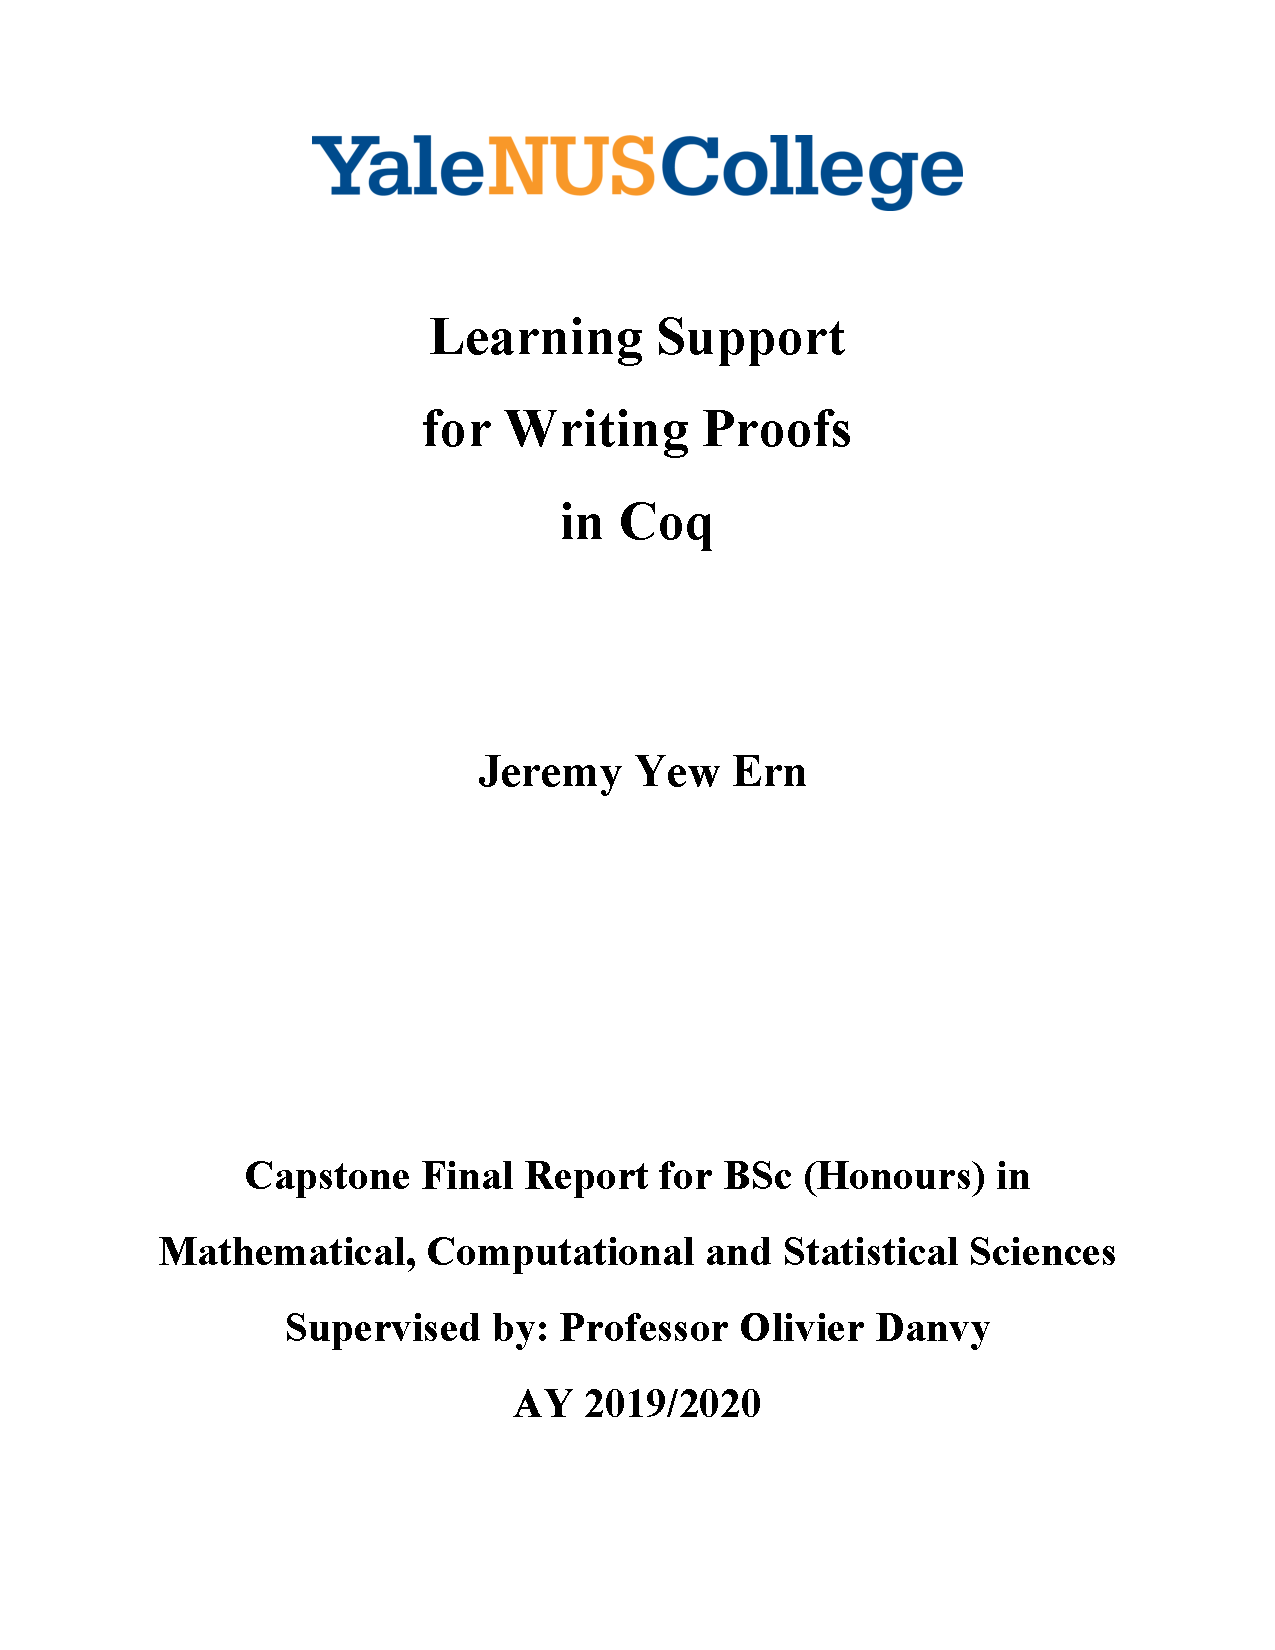
\includepdf[pages=-,pagecommand={},width=\textwidth]{titlepage.pdf}

\end{titlepage}

%----------------------------------------------------------------------------------------
%	DECLARATION & CONSENT
%----------------------------------------------------------------------------------------

% print, sign, and scan the declaration form, then include it here
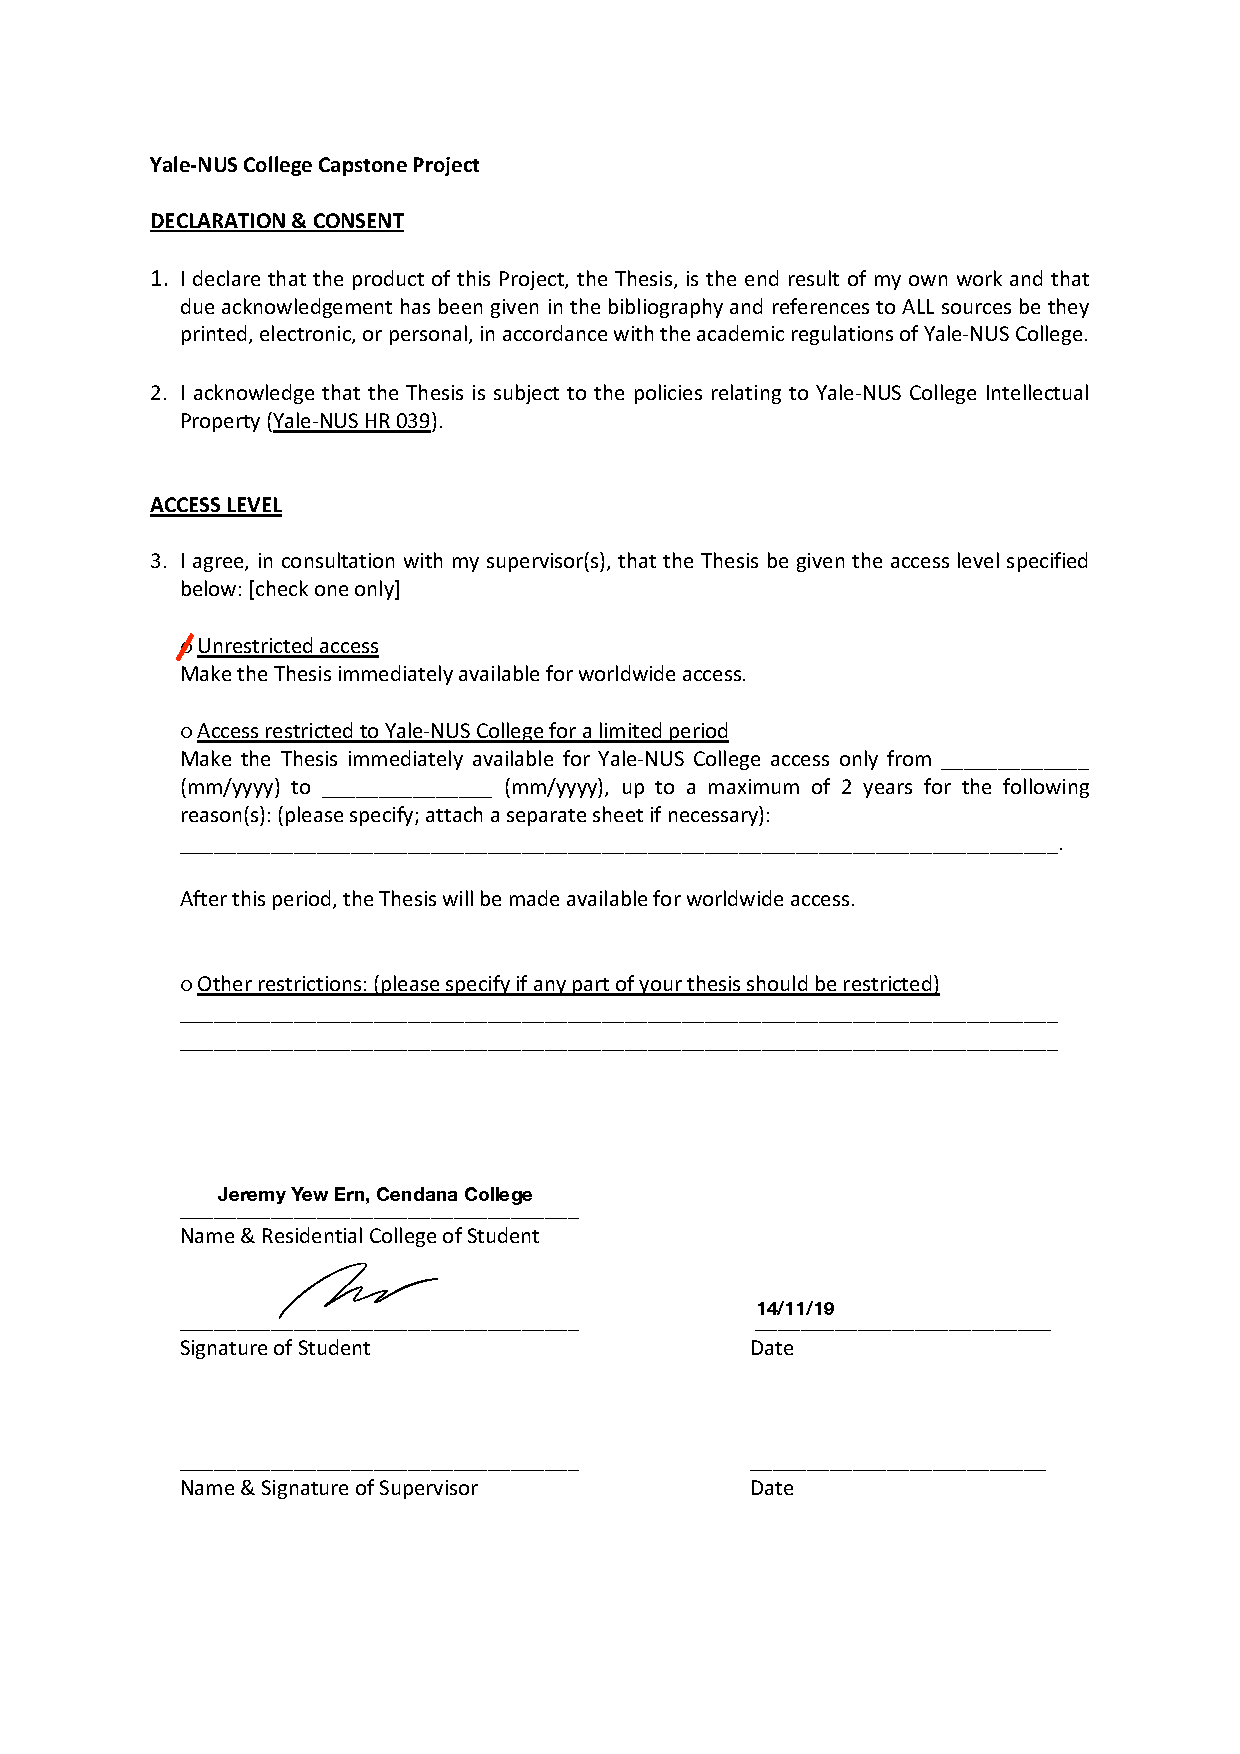
\includepdf[pages=-,pagecommand={},width=\textwidth]{declaration.pdf}

%----------------------------------------------------------------------------------------
%	ACKNOWLEDGEMENTS
%----------------------------------------------------------------------------------------

\begin{acknowledgements}
\addchaptertocentry{\acknowledgementname} % Add the acknowledgements to the table of contents
I would like to acknowledge Prof Danvy for his generous and dedicated guidance.
\end{acknowledgements}

%----------------------------------------------------------------------------------------
%	ABSTRACT PAGE
%----------------------------------------------------------------------------------------
 

\begin{abstract}
\addchaptertocentry{\abstractname} % Add the abstract to the table of contents
I provide learning support for students in YSC3236 Functional Programming and Proving (FPP), by building an interactive, Emacs-integrated tool that checks for syntax issues in student's Coq proof submissions. The tool thus acts as a set of 'safety rails' to guide students towards developing the proper muscle memory. The Lecturer will be able to provide a grammar specification as an input to the tool. 
\end{abstract}


%----------------------------------------------------------------------------------------
% CONTRIBUTIONS
%----------------------------------------------------------------------------------------

% \chapter{Claims}
%
% This paper presents the following original contributions:
%
% \begin{enumerate}
% 	\item A hardware device for haptic sensory substitution along with designs for the construction of such a system.
% 	\item Two implementations of sensory substitution using haptic feedback, continuous and delayed feedback-based spatial navigation tasks, each of which include:
% 		\begin{enumerate}
% 			\item a front-end for providing visual input to the user during the training phase with useful readouts to the researcher,
% 			\item a transmission protocol, which maps information from the task at hand (spatial coordinates, velocity information, etc) to time-based sensor actuation signals (20$^{\circ}$ on servo 1, 35$^{\circ}$ on servo 2, etc) in real-time.
% 		\end{enumerate}
% 	\item An evaluation framework for measuring the performance of a sensory substitution system, which provides sample tasks that can be used to standardise and compare performance across the board for future research.
% 	\item A review of existing hardware and software stacks as well as possible avenues for development based on the developed metrics.
% \end{enumerate}
%
% In addition, code for displaying results in real-time, modules for managing servo overload, network latency and other factors were also written by the author.


% %----------------------------------------------------------------------------------------
% %	DECLARATION PAGE
% %----------------------------------------------------------------------------------------
%
% \begin{declaration}
% \addchaptertocentry{\authorshipname} % Add the declaration to the table of contents
%
% \noindent I, \authorname, hereby declare that this Project, the Capstone Report and associated work listed herein, is the end result of my own work and that due acknowledgement has been given in the bibliography and references to ALL sources printed, electronic, or personal, in accordance with the academic regulations of Yale‐NUS College.
% I acknowledge that the Thesis is subject to the policies relating to Yale‐NUS College Intellectual  Property (Yale‐NUS HR 039).
%
%
% % I confirm that:
% %
% % \begin{itemize}
% % \item This work was done wholly or mainly while in candidature for a research degree at this University.
% % \item Where any part of this thesis has previously been submitted for a degree or any other qualification at this University or any other institution, this has been clearly stated.
% % \item Where I have consulted the published work of others, this is always clearly attributed.
% % \item Where I have quoted from the work of others, the source is always given. With the exception of such quotations, this thesis is entirely my own work.
% % \item I have acknowledged all main sources of help.
% % \item Where the thesis is based on work done by myself jointly with others, I have made clear exactly what was done by others and what I have contributed myself.\\
% % \end{itemize}
%
% \noindent Signed:\\
% \rule[0.5em]{25em}{0.5pt} % This prints a line for the signature
%
% \noindent Date:\\
% \rule[0.5em]{25em}{0.5pt} % This prints a line to write the date
% \end{declaration}
%
% \cleardoublepage

%----------------------------------------------------------------------------------------
%	QUOTATION PAGE
%----------------------------------------------------------------------------------------

% \vspace*{0.2\textheight}
%
% \noindent\enquote{\itshape Thanks to my solid academic training, today I can write hundreds of words on virtually any topic without possessing a shred of information, which is how I got a good job in journalism.}\bigbreak
%
% \hfill Dave Barry

%----------------------------------------------------------------------------------------
%	LIST OF CONTENTS/FIGURES/TABLES PAGES
%----------------------------------------------------------------------------------------

\tableofcontents % Prints the main table of contents

% \listoftables % Prints the list of tables
% \label{lst:tabs}

% \listoffigures % Prints the list of figures
% \label{lst:figs}
%----------------------------------------------------------------------------------------
%	ABBREVIATIONS
%----------------------------------------------------------------------------------------

% \begin{abbreviations}{ll} % Include a list of abbreviations (a table of two columns)
%
% \textbf{LAH} & \textbf{L}ist \textbf{A}bbreviations \textbf{H}ere\\
% \textbf{WSF} & \textbf{W}hat (it) \textbf{S}tands \textbf{F}or\\
%
% \end{abbreviations}

%----------------------------------------------------------------------------------------
%	PHYSICAL CONSTANTS/OTHER DEFINITIONS
%----------------------------------------------------------------------------------------

% \begin{constants}{lr@{${}={}$}l} % The list of physical constants is a three column table
%
% % The \SI{}{} command is provided by the siunitx package, see its documentation for instructions on how to use it
%
% Speed of Light & $c_{0}$ & \SI{2.99792458e8}{\meter\per\second} (exact)\\
% %Constant Name & $Symbol$ & $Constant Value$ with units\\
%
% \end{constants}

%----------------------------------------------------------------------------------------
%	SYMBOLS
%----------------------------------------------------------------------------------------

% \begin{symbols}{lll} % Include a list of Symbols (a three column table)
%
% $a$ & distance & \si{\meter} \\
% $P$ & power & \si{\watt} (\si{\joule\per\second}) \\
% %Symbol & Name & Unit \\
%
% \addlinespace % Gap to separate the Roman symbols from the Greek
%
% $\omega$ & angular frequency & \si{\radian} \\
%
% \end{symbols}

%----------------------------------------------------------------------------------------
%	DEDICATION
%----------------------------------------------------------------------------------------

%----------------------------------------------------------------------------------------
%	THESIS CONTENT - CHAPTERS
%----------------------------------------------------------------------------------------

\mainmatter % Begin numeric (1,2,3...) page numbering

\pagestyle{thesis} % Return the page headers back to the "thesis" style

% Include the chapters of the thesis as separate files from the Chapters folder
% Uncomment the lines as you write the chapters
% Chapter Template

\chapter{Introduction} % Main chapter title

\label{intro} % Change X to a consecutive number; for referencing this chapter elsewhere, use \ref{ChapterX}

%----------------------------------------------------------------------------------------
%	SECTION 1
%----------------------------------------------------------------------------------------

\section{Introduction}
The goal of this research project is to provide learning support for students enrolled in YSC3216: Functional Programming and Proving (FPP), by building a tool that checks for syntax issues in student's proof submissions.

FPP is a course in Yale-NUS College taught by Professor Olivier Danvy, under the Mathematical, Computational and Statistical Sciences major. FPP introduces students to the Coq proof assistant, which is a system for writing and verifying formal proofs. 

The learning goal for the first half of the course is to build muscle memory for basic proof techniques and programming habits. 

To this end, I implement a program that can act as a set of 'safety rails' to guide students towards developing the proper muscle memory. In particular, the program will enforce explicit tactic application within a subset of Coq, amongst other syntax rules. The Lecturer will be able to provide a grammar specification as an input to the tool. The program will be written as an extension of the Emacs text editor, and can therefore be used by students interactively. 
%-----------------------------------
%	SUBSECTION 1
%-----------------------------------
\section{Context}
\subsection{Functional programming (FP)}
Functional programming is a programming paradigm that models programs as mathematical functions. That is, a program defines a mapping of every possible input to exactly one output value. Functional programming is partly characterized by its 'declarative' style, in which the programmer directly expresses the desired output, derived from the input.

Students taking FPP are expected to have completed Intro to Computer Science taught in Yale-NUS, which trains them in functional programming with the language OCaml. Coq has a language of programs that is very similar to OCaml, and is in fact written in OCaml. 

\subsection{Proving}
In mathematics, a proposition is a statement that either holds or does not hold; a proposition is also sometimes called a theorem or lemma. 

Proofs can be defined as a logical argument about whether a proposition holds. Proofs use logical rules to demonstrate that what we are sure of (an axiom) implies the truth of something we were not sure of. 

In mathematical proofs, propositions often contain equations, which are statements asserting the equality of two expressions containing variables (unknown values). In equational reasoning, we apply axioms to equations in order to incrementally transform them into something that is clearly true. 

\subsection{Verifiable proofs with the Coq proof assistant}
Many proofs in mathematics or computer science are natural language proofs - that is, they are written in a natural language, like English. Even though they may use jargon and formal symbols, they may be considered informal. Since natural languages are often ambiguous, natural language proofs are susceptible to misinterpretation or misconception. Furthermore, informal proofs rely on humans to check for logical errors, but humans are fallible.

On the other hand, just as there programming languages that express a set of instructions to be executed by a computer, there are also domain-specific languages for writing formal proofs that can be automatically, or mechanically, verified by a computer. 

Therefore Coq allows us to write formal, verifiable proofs in a structured logical language called Gallina, and will also automatically verify that our proofs are correct. 

Proving is done as such: 
1. First, we state a theorem (or lemma, proposition, etc) in the logical language of Coq. 
2. Then, we solve 'subgoals'  generated by Coq (sub-statements we need to prove in order to prove the theorem) by stating a sequence of 'tactics' (the method we use at each step). As we apply each tactic to the current subgoal (by executing each line of code), Coq will progressively transform the subgoal.
3. Once all our subgoals have been transformed into something that is clearly true, our proof is complete. Every proof step has been demonstrated to progress logically from each other; this process can be reproduced by any other user executing the same proof. Thus the the proof is verifiably correct. 


\subsection{YSC3236 Functional Programming and Proving (FPP)}
FPP is a course in Yale-NUS College taught by Professor Olivier Danvy, under the Mathematical, Computational and Statistical Sciences major. The class is taken not only by Yale-NUS students, but also PhD and post-doctoral students from the National University of Singapore (NUS) School of Computing (SoC). 

FPP introduces students to the Coq proof assistant. Through the course, students gain an appreciation for the interconnectedness of computer programs and logical proofs - which have previously been presented to them as distinct domains of knowledge. For example, they are led to realize that an explicitly written Coq proof exactly corresponds to an equivalent mathematical proof they have written in detail, by hand.
  
Students engage in weekly assignments consisting of rigorous, progressive exercises involving:
\begin{itemize}    
    \item writing mathematical proofs
    \item  writing programs, and proofs about the properties of programs
    \item eventually, stating their own theorems and proving them
\end{itemize}

\subsection{GNU Emacs Editor}   

Emacs is a family of real-time text editors which are characterized by their customizability and extensibility. GNU Emacs was written in 1984 by GNU Project founder Richard Stallman. 

The user interacts with files displayed in 'buffers' - a view of a text file - via **commands** invoked by 'macros' - keystroke sequences. Feedback and status messages are displayed in a smaller buffer at the bottom of the screen - the 'minibuffer'. The user can create and dismiss buffers, and multiple buffers can exist without all being on display.  

\begin{itemize}
    \item Emacs is customizable because users can change the behaviour of some commands via parameters, without having to redefine or modify the underlying code of the command itself. Users can also easily redefine key mappings.
    \item Emacs is extensible because users can write new commands as programs and bind them to new macros. 
    \item GNU Emacs provides a language based on Lisp, Emacs Lisp, that is used to write extensions/programs run within Emacs. 
\end{itemize}

GNU Emacs is used in Intro CS, Intro to Algos and Data Structures, and FPP, so students are expected to have familiarity with its interface and indeed will be required to use it, since the class uses the Proof General interface. 


\subsection{Proof General}   
Proof General is a powerful, configurable and generic Emacs interface for proof assistants, developed at the University of Edinburgh since 1992. It provides a common interface across various proof assistants, including Coq, and allows users to interactively edit proof scripts. 

The interface presents users with three buffers (windows): one buffer in which the Coq script is to edited, one buffer to display subgoals, and one buffer to display other responses like search results or error messages.
% Chapter Template

\chapter{Building muscle memory} % Main chapter title

\label{building-muscle-memory} % Change X to a consecutive number; for referencing this chapter elsewhere, use \ref{ChapterX}

%----------------------------------------------------------------------------------------
%	SECTION 1
%----------------------------------------------------------------------------------------

\section{A skilled discipline}
The learning philosophy of FPP is that programming and proving is similar to training in any skilled discipline such as martial arts, cooking, or dance: beginner training should build muscle memory for basic skills and habits. 

For example, if you are training to be a chef, but you don't develop proper knife skills early on, this will hurt you for the rest of your career. 

Therefore, in the first half of the course, students complete rigorous, progressive exercises in order to practice specific proof techniques and programming habits. In the second half of the course, students can then rely on this muscle memory to write proofs with greater creativity and efficiency. By the end of the course, students will have independently written more proofs than they have ever written in their lives, and all of these proofs would have been verified by Coq.

% Chapter Template

\chapter{Writing proofs} % Main chapter title

\label{writing-proofs} % Change X to a consecutive number; for referencing this chapter elsewhere, use \ref{ChapterX}

%----------------------------------------------------------------------------------------
%	SECTION 1
%----------------------------------------------------------------------------------------

\section{What could go wrong?}
With programming languages, there are usually many ways to write the same program. In the same way, there are many equivalent representations of a Coq proof, because Coq is flexible and allows you to take shortcuts. However, for new learners, this flexibility can be counterproductive. In the context of FPP, several issues arise. 

\subsection{Abuse of tactics}
First, students may abuse tactics that have not been introduced in the course. 

When students get stuck on a proof, they might Google for related solutions or search the Coq documentation for anything that will 'solve' the proof. They might end up using a magical tactic, for example `trivial`, as in the latter version of the example proof below. 
\begin{verbatim}
Lemma SSSn_is_3_plus_n :
  forall n : nat,
  S (S (S n)) = 3 + n.
Proof.
  intro n.
  rewrite <- (Nat.add_1_l n).
  rewrite <- (plus_Sn_m 1 n).
  rewrite <- (plus_Sn_m 2 n).
  reflexivity.
Qed.
\end{verbatim}

\begin{verbatim}
Lemma SSSn_is_3_plus_n :
  forall n : nat,
  S (S (S n)) = 3 + n.
Proof.
  trivial.
Qed.
\end{verbatim}

Under the hood, the `trivial` tactic uses some heuristics to automatically try various strategies to solve the current formula. However, in the first half of the course the focus is for students to understand every single proof step they write, because if students cannot explain what they are doing, they do not really understand it. Therefore, using a tactic like `trivial` completely goes against the objective of the exercise. 

Yet these tactics still appear in student submissions, because they might still have the bad programmer mindset of "if it works, its fine". This causes time between resubmissions to be wasted on superficial feedback. 

\subsection{ Misuse of tactics }
Second, even when students use tactics that have been introduced, they may misuse them by taking shortcuts.

For instance, the rewrite tactic is used to apply a rule to the current formula. A rewrite rule is a function that expects specific terms in the formula as arguments; Coq will rewrite the given terms. For example, the rewrite rule below accepts three arguments, n, m, p.

\begin{verbatim}
Check Nat.add_assoc.
# Nat.add_assoc : forall n m p : nat, n + (m + p) = n + m + p. 
\end{verbatim}

However, Coq is flexible with the number of arguments you give it. As the example proofs below demonstrate, you could give the rewrite rule three, two, one or zero of the rewrite arguments required, and Coq will simply pick the first terms in the formula that it can apply the rule to. 
\begin{verbatim}
Proposition add_assoc_nested :
  forall a b c d e: nat,
    a + b + c + d + e = 
    a + (b + (c + (d + e))).
Proof.
  intros a b c d e.
  rewrite -> (Nat.add_assoc a b (c + (d + e)) ).
  rewrite -> (Nat.add_assoc (a + b) c (d + e) ).
  rewrite -> (Nat.add_assoc (a + b + c) d e ).
  reflexivity.
Qed.
\end{verbatim}
\begin{verbatim}
Proposition add_assoc_nested :
  forall a b c d e: nat,
    a + b + c + d + e = 
    a + (b + (c + (d + e))).
Proof.
  intros a b c d e.
  rewrite -> (Nat.add_assoc a b )
  rewrite -> (Nat.add_assoc (a + b) ).
  rewrite -> Nat.add_assoc.
  reflexivity.
Qed.
\end{verbatim}
However, in the first half of the course, the focus is on understanding the proof at a low level. Clearly, students need to be aware of exactly which terms they have changed at every step. Otherwise, they may get stuck in a proof because they applied a rewrite rule to the wrong term, or they might reach a solution without knowing how. Therefore, taking advantage of this shortcut goes against the spirit of the exercise. 

Furthermore, this issue is not easy to check manually, especially with assignments that are hundreds of lines long.

These two issues - abuse and misuse of tactics - correspond to issues of **abstract syntax** (what language constructs are represented in the grammar) and **concrete syntax** (what structures are used to represent language constructs) respectively. 

Therefore, it would be nice to have a system that can anticipate and identify both abstract and concrete syntax issues, to save both students and the Lecturer's time and help achieve the learning goals of the course.   


\subsection{Other issues}
Other issues I have discussed with the Lecturer include: 
\begin{itemize}
  \item arbitrary indentation levels for proof subcases 
  \item inconsistent naming
  \item breaking style conventions. 
\end{itemize}


All these issues seem to persist across the progression of the module, as well as iterations of the module, despite the Lecturer explaining to the students the rationale for following provided syntactical guidelines, and repeated reminders.

The idea is for the proposed tool to cut down on the amount of **'superficial'** feedback - e.g., 'don't use this tactic, because...', or 'this is bad style, please correct it in this way', etc. - that the Lecturer must give repeatedly to individual students, and instead automatically lead students towards solutions that only require **substantive** feedback - e.g., ideas to pursue, possible restructuring of the proof, etc. The less superficial feedback is required, the more time the Professor can spend on providing substantive feedback. Also, students will spend less effort correcting style errors if they do so immediately.

Yet, superficial feedback is not merely incidental. Superficial feedback reflects the formal concerns of the course and helps reinforces good programming habits, which will not only assist the learning experience of students, but benefit them in future endeavors. Therefore, the tool does not simply emphasize pedantic concerns; it makes concrete the formal training prescriptions of the course. 
% Chapter Template

\chapter{Solution} % Main chapter title

\label{solution} % Change X to a consecutive number; for referencing this chapter elsewhere, use \ref{ChapterX}

%----------------------------------------------------------------------------------------
%	SECTION 1
%----------------------------------------------------------------------------------------


\section{A grammar of grammars}
The solution to these issues of abstract and concrete syntax is to develop a system that enforces explicit tactic application within a subset of Coq, amongst other rules. This system will be in the form of a program that takes as input a student's Coq file, as well as a grammar specification provided by the Lecturer. It will output warnings about instances where a syntax rule has been violated. (From here, I refer to 'the program' interchangeably as 'the tool' or 'the parser'.)

The program will be writen as an extension of the Emacs editor, so students can execute a command within Emacs to parse the current file, and thus use the tool interactively as they construct their proofs. 

The program will thus act as a set of safety rails for students to develop the right habits, in the spirit of learning for the first half of the course. As a result, students will have earlier, automated intervention on syntactical issues in their assignments, and the Lecturer can spend more time on substantive rather than superficial feedback. 

However, the parser should not 'hard-code' a grammar that only enforces particular syntax rules. Instead, it should accept and parse a grammar specification that is readable and easily editable, and enforce that grammar. In other words, we need to implement a grammar of grammars. This will allow the Lecturer to modify existing rules or extend them, without having to modify the source code of the parser. This will also make it easier for other course instructors or developers to modify the parser behaviour for their own needs. 

\section{Implementation trade-offs}
The first trade-off is whether to write a custom syntax parser by hand, or to use a parser generator.

A parser generator is a program that accepts a grammar specification as input, and automatically generates a parser that implements the grammar. I have identified parser generators intended to be run within Emacs, and written in Emacs Lisp (more on that below).

A parser generator would be ideal - we do not want to reinvent the wheel. Firstly, in theory, there is minimal to no programming to be done. Instead, we declare a grammar using some notation. 

Secondly, relying only on the declared grammar makes the program more extensible; it is easier for the Lecturer or other developers to modify existing rules or add new rules, since they do not need to touch underlying code.

However, it will be necessary to grasp the grammar that is required as input in the first place. 

A second trade-off relates to the case where we write a custom parser by hand: whether to write it using Emacs Lisp, or another language that I am more familiar with.

Of course, using a familiar language might mean that we get to a first working version faster. But an Emacs Lisp implementation has many benefits: 
\begin{itemize}
    \item Easier for other Emacs developers to build on  
    \item Integrated with Emacs editor features
    \item Run within Emacs. No need to call external process, no external dependencies, no interoperability issues (e.g. making a call to create a new thread, etc).  
\end{itemize}


This is why it is ideal to use a parser generator that generates Emacs Lisp code.  

\section{Current progress}
I have made progress in the following areas: 

\begin{itemize}
    \item Defining a subset of Coq grammar.
    \item Exploring different types of parsers for different types of languages.
    \item How to write a parser.
    \item How to write Emacs Lisp programs.
    \item How to write an Emacs extension.
\end{itemize}


In particular, I have written a script in Emacs Lisp that registers an Emacs interactive command, which may be executed while editing a Coq proof. The command is able to take the current buffer and use the Coq shell to parse it for Coq syntax errors. This command would be eventually used to run our custom parser; the idea is to first check that the input is syntactically correct with respect to Coq's grammar. This allows us to develop our custom parser assuming that the input code is already syntactically correct, hence we may define or provide a grammar that only encompasses a subset of Coq's grammar.

Additionally, I have also started trying to use the Semantic Bovine parser generator. Semantic is a framework for writing Emacs packages, and Bovine is a built-in parser generator provided by Semantic. It accepts a BNF (Backus-Naur Formation)-like grammar specification, and generates a parser in Emacs Lisp, which is ideal. The main obstacle for now would be the slightly obscure documentation. The first step I am aiming for would be to specify a simple grammar (such as for arithmetic expressions with infix notation), and ensure that it raises an appropriate error when given a syntactically incorrect input. 

\section{Challenges ahead}
The challenges ahead would be to decide on and proceed with an implementation of a program that can enforce a grammar addressing the two issues mentioned. Following which, I can then explore other rules mentioned. I will also be iterating on the tool based on usability feedback from both the Lecturer and FPP students, and the feedback will also be the measure of success for my project.


%----------------------------------------------------------------------------------------
%	BIBLIOGRAPHY
%----------------------------------------------------------------------------------------

% \printbibliography[heading=bibintoc]
%----------------------------------------------------------------------------------------
%	THESIS CONTENT - APPENDICES
%----------------------------------------------------------------------------------------

\chapter{References} % Main chapter title

\appendix % Cue to tell LaTeX that the following "chapters" are Appendices

% Include the appendices of the thesis as separate files from the Appendices folder
% Uncomment the lines as you write the Appendices

 % Appendix A

\chapter{Frequently Asked Questions} % Main appendix title

\label{AppendixA} % For referencing this appendix elsewhere, use \ref{AppendixA}

\section{How do I change the colors of links?}

The color of links can be changed to your liking using:

{\small\verb!\hypersetup{urlcolor=red}!}, or

{\small\verb!\hypersetup{citecolor=green}!}, or

{\small\verb!\hypersetup{allcolor=blue}!}.

\noindent If you want to completely hide the links, you can use:

{\small\verb!\hypersetup{allcolors=.}!}, or even better: 

{\small\verb!\hypersetup{hidelinks}!}.

\noindent If you want to have obvious links in the PDF but not the printed text, use:

{\small\verb!\hypersetup{colorlinks=false}!}.


%----------------------------------------------------------------------------------------

\end{document}
